\documentclass[11pt]{article}
\usepackage[margin=2.2cm]{geometry}
\usepackage{graphicx,booktabs,caption,float,amsmath}
\captionsetup{font=small}
\title{CS6600 Assignment 3: Dynamic Scheduling (Tomasulo) Simulator}
\author{Shubham Jadhav (CS24S009)}
\date{}
\begin{document}
\maketitle

\section{Simulator and validation}
\texttt{proj\_tomasulo.cpp} models fetch, dispatch (IF/ID), scheduling queue (IS), execute (EX) and writeback (WB) for an out-of-order machine that fetches, dispatches and issues up to $N$ instructions per cycle. The dispatch queue holds $2N$ entries and the scheduling queue $S$. Source operands are renamed at dispatch through a 128-entry register file of \{tag, ready\}; ready instructions issue oldest first, up to $N$ per cycle; operation types 0, 1 and 2 take 1, 2 and 10 cycles; a finishing instruction broadcasts its tag and marks the register ready only if the register still maps to its tag. Both validation runs (gcc $N{=}8$, $S{=}64$; perl $N{=}3$, $S{=}16$) match the reference output for all 10{,}000 instructions under \texttt{diff -iw}. The model has perfect caches and branch prediction, so the only limits on IPC are the true data dependences, the width $N$, and the sizes of the two queues.

\section{IPC versus scheduling queue size}
\begin{figure}[H]\centering
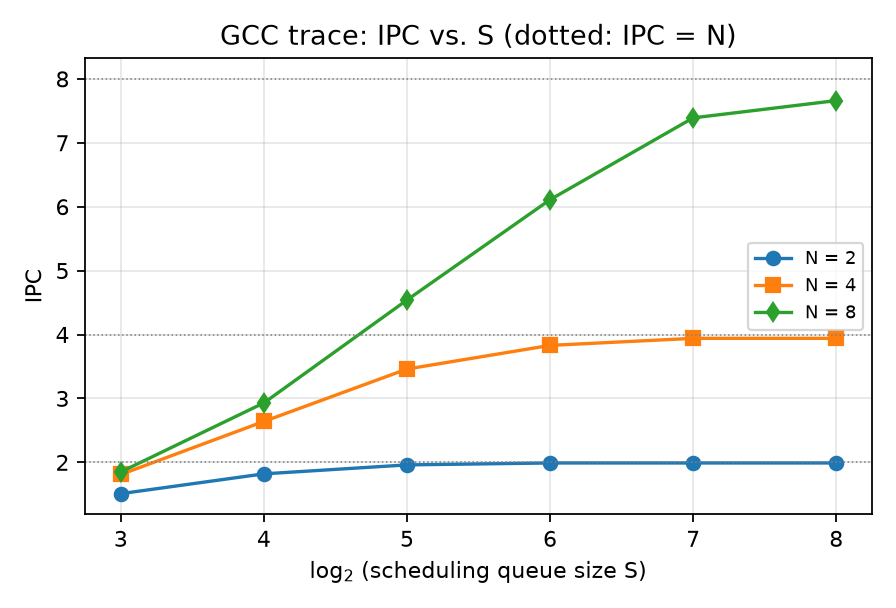
\includegraphics[width=.49\linewidth]{GCC_Benchmark.png}\hfill
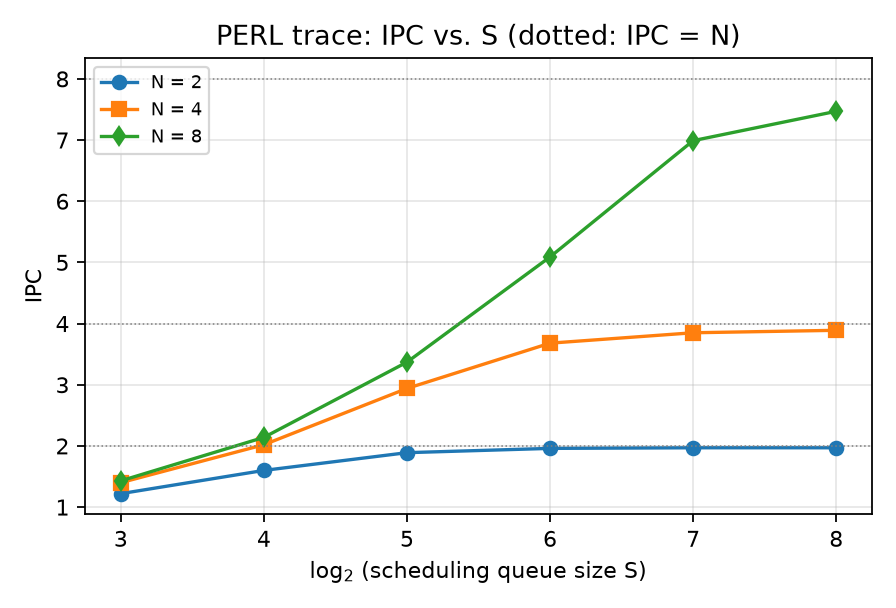
\includegraphics[width=.49\linewidth]{PERL_Benchmark.png}
\caption{IPC versus the scheduling queue size $S$ for $N=2,4,8$ (dotted lines mark IPC $=N$).}
\end{figure}
\begin{center}\small\begin{tabular}{llcccccc}\toprule
Trace & $N$ & $S=8$ & 16 & 32 & 64 & 128 & 256\\\midrule
gcc & 2 & 1.51 & 1.82 & 1.96 & 1.99 & 1.99 & 1.99\\
gcc & 4 & 1.81 & 2.64 & 3.46 & 3.83 & 3.94 & 3.94\\
gcc & 8 & 1.85 & 2.93 & 4.54 & 6.11 & 7.39 & 7.66\\
perl & 2 & 1.22 & 1.60 & 1.89 & 1.96 & 1.97 & 1.97\\
perl & 4 & 1.40 & 2.02 & 2.94 & 3.68 & 3.85 & 3.89\\
perl & 8 & 1.43 & 2.14 & 3.37 & 5.09 & 6.99 & 7.47\\\bottomrule
\end{tabular}\end{center}

\subsection*{1. Trend in IPC as $S$ grows}
IPC rises with $S$ and then saturates, with sharply diminishing returns: for gcc at $N=4$ doubling $S$ from 8 to 16 adds 0.83 IPC, from 32 to 64 adds 0.37 and from 64 to 128 only 0.11. The mechanism is only the scheduling window. A larger queue lets the scheduler look farther ahead of the oldest unfinished instruction, finding independent instructions to issue while long-latency (10-cycle) instructions and their dependants wait, so it exposes more instruction-level parallelism. It saturates when the window is big enough that all the parallelism the program offers within the width limit is already visible. Little's law confirms this: the occupancy of the queue equals IPC times the average time an instruction spends in it. For gcc, $N=8$, $S=64$ this is $6.11\times10.3\approx 63$, so the queue is full and IPC is $S$-limited; at $S=256$ it is $7.66\times20.8\approx159<256$, so the queue is no longer the limit. (There are no caches or contending units in this model, so S does not interact with cache misses or functional-unit contention; IPC cannot fall when $S$ grows.)

\subsection*{2. Trend in IPC as $N$ grows}
IPC grows with $N$ at large $S$ and approaches $N$ when the window is large enough: gcc reaches 1.99, 3.94 and 7.66 for $N=2,4,8$ at $S=256$ (99.5\%, 98.5\% and 96\% of $N$); perl reaches 98.5\%, 97\% and 93\%. It never exceeds $N$, because fetch, dispatch and issue are $N$ wide. The efficiency drops as $N$ grows (perl 93\% at $N=8$), because wider issue needs more independent instructions in the window every cycle and dependence chains (each 10-cycle operation delays all of its dependants) become the limit. At small $S$ a wider machine barely helps: for gcc at $S=8$, IPC is 1.51, 1.81 and 1.85 for $N=2,4,8$.

\subsection*{3. Interaction between $S$ and $N$}
The two limits combine as roughly $\mathrm{IPC}\approx\min(N,\;S/\text{residency})$. In the \emph{S-limited} regime (small $S$), the curves for different $N$ nearly coincide because a full queue cannot feed more than $S/\text{residency}$ instructions per cycle: at $S=8$ the $N=4$ and $N=8$ results differ by 0.04 IPC for gcc and by 0.03 for perl. In the \emph{N-limited} regime (large $S$) the curves separate and flatten at $N$. The $S$ needed for saturation grows in proportion to $N$: IPC reaches 98\% of its maximum at $S=32$--64 for $N=2$, $S=128$ for $N=4$, and has not yet saturated at $S=256$ for $N=8$ (7.39 $\to$ 7.66). Equivalently, to keep $N$ instructions per cycle issuing, the queue must hold about $N$ times the average residency (20--28 cycles in these traces at S=256), so a wide machine needs a proportionally larger scheduling queue, and a large queue is useless on a narrow machine ($N=2$ gets nothing from $S>64$).

\end{document}
